\section{Sensores Indutivos}
\label{sec:indutivo}

Como apresentado por \citeonline{INSTRUME}, sensores indutivos são dispositivos sem contato e utilizados geralmente 
para medição de posição. Utilizando o efeito de indução eletromagnética em um corpo condutor, é possível produzir 
corrente elétrica quando o campo magnético é variável ou quando é efetuado movimento em um campo estático. Considerando uma espira 
C, a corrente induzida pode ser representada por \cite{moyses}:

\begin{equation}
  i = \frac{-1}{R} \frac{d \Phi_c}{dt},
  \label{eq:I_indu}
\end{equation}
onde i é a corrente induzida, R é a resistência de uma espira C, e $\frac{d \Phi_c}{dt}$ é a variação de campo que atravessa a 
espira C. A existência dessa corrente na espira está associada uma força eletromotriz (fem) induzida descrita por \cite{moyses}:

\begin{equation}
  \varepsilon = Ri = -\frac{d\Phi_c}{dt},
  \label{eq:fem_ind}
\end{equation}
em que $\varepsilon$ é a fem induzida.
 
 Como neste trabalho são utilizadas pares de bobinas geradoras e sensoras é utilizado o efeito de indução mútua que é 
apresentado por \citeonline{Young}. Considerando duas bobinas vizinhas (vide Figura \ref{fig:Duasbob}). Uma corrente $i_1$ 
circulando na bobina 1 produz campo magnético \textbf{$\overrightarrow{B}$} e um fluxo magnético através da bobina 2. Quando 
$i_1$ varia, o fluxo magnético através da bobina 2 também varia, produzindo uma fem.

\begin{figure}[H]
	\vspace{4mm}
  \centering
  \caption{Exemplo de efeito de indução mútua}
  \label{fig:Duasbob}
  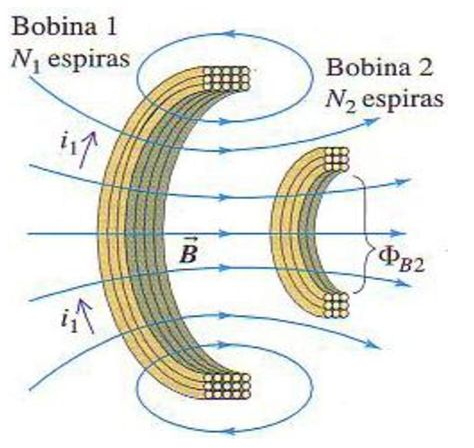
\includegraphics[scale=0.3]{imagens/InducaoMutua.png}
  \caption*{Fonte: \citeonline[p. 317]{Young}.}
\end{figure}


  A fem induzida na bobina 2 pode ser representada em termos da variação de corrente na bobina 1, conforme \cite{Young}:

\begin{equation}
  \varepsilon_2 = -M \frac{di_1}{dt},
  \label{eq:variacao}
\end{equation}
 onde $M$ é conhecida como indução mútua e depende das indutâncias das bobinas 1 e 2, assim como do acoplamento entre elas. Em 
termos de fluxos magnéticos, a indutância mútua pode ser obtida a partir de \cite{Young}:

\begin{equation}
  M =\frac{ N_2 \Phi_{B2}}{i_1} =  \frac{N_1\Phi_{B1}}{i_2},
 \label{eq:indutanciaMutua}
\end{equation}

em que $N_1$ e $N_2$ são os número de espiras das respectivas bobinas, $\Phi_{B1}$ e $\Phi_{B2}$ correspondem aos fluxos magnéticos nas bobinas 1 e 2 respectivamente, $i_1$ e $i_2$ são as correntes de cada uma das bobinas. 

Este princípio da indução é aplicado em transformadores, com circuitos CA para aumentar ou diminuir uma tensão de entrada. Um dos 
problemas 
envolvidos em transformadores é que a potência fornecida pela bobina fonte depende da resistência da fonte de carga do circuito 
conectado a outra bobina \cite{Young}.

Para solucionar este problema, considera-se a condição de ressonância, onde a impedância atinge o seu valor mínimo e a corrente 
atinge o valor máximo. Para isso, é necessário adicionar um capacitor ao circuito da bobina. Desta forma, a frequência de ressonância
do circuito LC é dada por:
\begin{equation}
  f_0 = \frac{1}{2 \pi \sqrt{LC}},
 \label{eq:freqResso}
\end{equation}
$L$ é o indutor e $C$ é o capacitor. A Figura \ref{fig:transform} demonstra o 
esquemático do sensor e gerador projetados para operar em ressonância.\\


\begin{figure}[H]
  \centering
 	\vspace{4mm}
 	    \caption{Topologia dos circuitos de sensoriamento}
 	    \label{fig:transform}
    \begin{circuitikz} 
      \draw
      %circuito esquerda
      (0,0) to [short] (2,0)
      to [C, l_=$C_2$] (2,2)
      to [short] (0,2)
      (2,0) to [short] (4,0)
      to [L,l_=$L_2$] (4,2)
      to [short] (2,2)


      %circuito direita
      (6,2) to [R,l=$R_1$] (8,2)
      to [C, l=$C_1$] (10,2)
      (6,2) to [L, l=$L_1$] (6,0)
      to [short] (10,0)
      ;

      \draw [decorate, decoration={brace, amplitude=10pt, mirror, raise=4pt}, yshift=0pt] (0,0) -- (4,0)  node 
      [midway, yshift=-0.8cm]{sensor};
      \draw [decorate, decoration={brace, amplitude=10pt, mirror, raise=4pt}, yshift=0pt] (6,0) -- (10,0) node 
      [midway, yshift=-0.8cm] {gerador};
    \end{circuitikz}
	
    \caption*{Fonte: \citeonline[p. 67]{RUANI}.}

\end{figure}

Para o projeto do valor de $C$, foi assumida a frequência de ressonância pré-definida de $100\textrm{ }kHz$ e a indutância das bobinas desenvolvidas por 
\citeonline{RUANI}. Isolando-se $C$ em \ref{eq:freqResso} obtem-se:	

\begin{equation}
 C = \frac{1}{4 \pi^2 f_0^2 L}.
 \label{eq:capa}
\end{equation}
